\documentclass[a4paper,11pt]{article}

%%%%%%%%%%%%%%%%%%%%%%%%%%%%%%%%%%%%%%%%%%%%%%%%%%%%%%%%%%%%%%%%%%%%%%
%%% packages (and their customizations)
%%%%%%%%%%%%%%%%%%%%%%%%%%%%%%%%%%%%%%%%%%%%%%%%%%%%%%%%%%%%%%%%%%%%%%
\usepackage[utf8]{inputenc}
\usepackage{hyperref}
\usepackage{authblk}
\usepackage{amsmath}
\usepackage{amsthm}
\usepackage{amsfonts}
\usepackage{fullpage}
\usepackage[tt=false]{libertine}
\usepackage{xifthen}
\usepackage[x11names,rgb]{xcolor}
\usepackage{fixme}
\fxsetup{status=draft, theme=color, layout={inline}}
\renewcommand{\fixmelogo}{\textcolor{black}{\colorbox{Firebrick1}%
    {\textsf{\textbf{FIX}}}}}
\usepackage{url}
\urlstyle{same}                 % same font as in text
\usepackage{booktabs}
\usepackage{setspace}
\usepackage{tikz}
\usepackage{mathtools}
\mathtoolsset{showonlyrefs}

\newcommand{\tk}{\tilde{k}}

% bibliography
\usepackage[style=authoryear]{biblatex}
\addbibresource{./bibliography.bib}

%%%%%%%%%%%%%%%%%%%%%%%%%%%%%%%%%%%%%%%%%%%%%%%%%%%%%%%%%%%%%%%%%%%%%%
%%% general macros
%%%%%%%%%%%%%%%%%%%%%%%%%%%%%%%%%%%%%%%%%%%%%%%%%%%%%%%%%%%%%%%%%%%%%%

\begin{document}

\title{``Exact present solution'' in continuous time}
\author{Tam\'as K.~Papp\thanks{\url{tkpapp@gmail.com}}}
\date{\today}
\maketitle

\begin{abstract}
  A small experiment that I performed to understand the method of \textcite{den2015exact}, which I wrote up as a tutorial with a small program in \textsc{Julia} \parencite{bezanson17:_julia}.
\end{abstract}

\begin{center}
\fbox{See the associated repository at \url{https://github.com/tpapp/exact-present} for the code.}
\end{center}
\paragraph{Setup.} Consider a deterministic Ramsey model in continuous time, with CRRA utility function (IES $\theta$), discount rate $\rho$, production function
\begin{equation}
  F(k) = A k^\alpha - \delta k
\end{equation}
and capital accumulation equation
\begin{equation}
  \label{eq:capital-accumulation}
  \dot{k}_t = F(k_t) - c_t
\end{equation}
The most frequently used form of the Euler equation is\footnote{Eg see \textcite[Chapter 8]{acemoglu2008introduction}.}
\begin{equation}
  \label{eq:Euler-equation-t}
  \frac{\dot{c}_t}{c_t} = \frac{1}{\theta} \bigl( F'(k_t) - \rho \bigr)
\end{equation}
First, we rewrite this into a recursive form. We are solving for the policy function $c(k)$, and thus
\begin{equation}
  \dot{c} = c'(k) \dot{k} = c'(k) \bigl( F(k) - c(k) \bigr)
\end{equation}
where we have used \eqref{eq:capital-accumulation} and dropped time indices. Plugging into~\eqref{eq:Euler-equation-t}, we obtain
\begin{equation}
  \label{eq:Euler-elasticity}
  \frac{c'(k)}{c(k)} \bigl( F(k) - c(k) \bigr) = \frac{1}{\theta} \bigl(F'(k)-\rho\bigr)
\end{equation}
We cast this into the form
\begin{equation}
  \label{eq:Euler-equation}
  c'(k) \bigl( F(k) - c(k) \bigr) = \frac{1}{\theta} \bigl(F'(k)-\rho\bigr) c(k)
\end{equation}
which should be easier to manipulate. We are looking for the solution $c(k)$ to \eqref{eq:Euler-equation}.

\paragraph{Methodology.} The key to the method outlined in \textcite{den2015exact} is the following:
\begin{enumerate}
\item fix $k$,
\item assume a functional form for $c(k)$ around this point,
\item solve \eqref{eq:Euler-equation} by imposing that this form holds locally.
\end{enumerate}
For simplicity, we choose a linear form
\begin{equation}
  \label{eq:linear-c}
  c(\tk) = c_0(k) + c_1(k)(k-\tk)
\end{equation}
First, from \eqref{eq:Euler-equation} and \eqref{eq:linear-c} we obtain
\begin{equation}
  \label{eq:linear-Euler}
  c_1(k)\bigl( F(k) - c_0(k) \bigr) = \frac{1}{\theta}\bigl( F'(k) - \rho \bigr) c_0(k) 
\end{equation}
Implicit differentiation by $k$ yields
\begin{equation}
  \label{eq:implicit}
  c'_1(k)\bigl( F(k) - c_0(k) \bigr) + c_1(k)\bigl( F'(k) - c'_0(k) \bigr) =
  \frac{1}{\theta}\biggl[ F''(k) c_0(k) + \bigl( F'(k) - \rho \bigr) c'_0(k) \biggr]
\end{equation}
Then we impose that the approximation is valid locally around $k$:
\begin{equation}
  \label{eq:validity}
  c'_0(k) = c_1(k)
  \qquad
  c'_1(k) = 0
\end{equation}
The first equation in \eqref{eq:validity} imposes that when we change $k$ a bit, we move along the tangent, while the second states that the tangent remains the same. \emph{This is a crucial assumption}, as it basically imposes no curvature. The performance of the method will depend on how good an approximation this is.

Using~\eqref{eq:validity}, \eqref{eq:implicit} becomes
\begin{equation}
  \label{eq:implicit-simple}
  c_1(k)\bigl( F'(k) - c_1(k) \bigr) = \frac{1}{\theta}\biggl[ F''(k) c_0(k) + \bigl( F'(k) - \rho \bigr) c_1(k) \biggr]
\end{equation}
For each $k$, we solve the system of \eqref{eq:linear-c} and \eqref{eq:implicit-simple}. 
Note that \eqref{eq:implicit-simple} still takes the curvature of $F$ into account.

\paragraph{Practicalities.}

Note that the system \eqref{eq:linear-Euler} and \eqref{eq:implicit-simple} is quadratic. Using random starting points, I mostly found  \emph{three} solutions: the right one ($c_1(k), c_0(k) > 0$), a trivial one $c_1(k) = c_0(k) = 0$, and a bogus one (with $c_1(k) < 0$). Consequently, reformulating the problem and using initial guesses is beneficial. Using \eqref{eq:Euler-elasticity} rules out the zero solution.

Let $k_s, c_s$ denote steady state capital and consumption. Initial guesses for the nonlinear optimizer are chosen as follows:
\begin{enumerate}
\item for a $k$ near $k_s$, $c_0(k), c_1(k) = c_s, F'(k_s)$.
\item for other $k$, find a nearby $\tk$ for which we have solved the problem, and use $c_0(\tk), c_1(\tk)$.
\end{enumerate}

\paragraph{Solution.}

Figure~\ref{fig:policy} shows the policy function. Figure~\ref{fig:policy-tangents} shows the same function, but with tangents drawn using $c_0(k)$ and $c_1(k)$. Note that the approximation is not exact, but evaluating its accuracy is beyond the scope of this short note. However, it could serve as a great initial guess, obtained at a very small computational price.

\begin{figure}
  \centering
  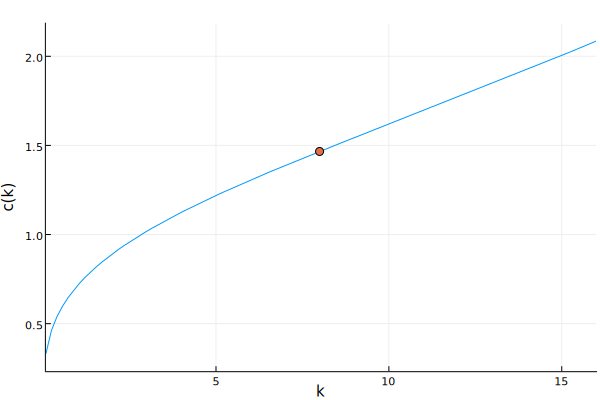
\includegraphics[width=0.9\textwidth]{../fig/ck.pdf}
  \caption{Policy function (steady state as a dot).}
  \label{fig:policy}
\end{figure}

\begin{figure}
  \centering
  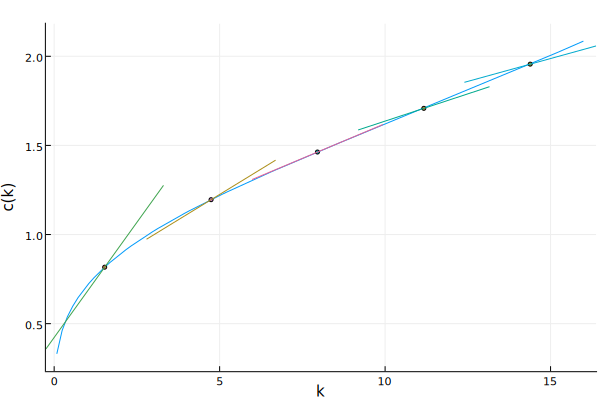
\includegraphics[width=0.9\textwidth]{../fig/ck-tangents.pdf}
  \caption{Policy function, with tangents drawn according to $c_1(k)$.}
  \label{fig:policy-tangents}
\end{figure}

\clearpage
\printbibliography

\end{document}

% Local Variables:
% reftex-default-bibliography: ("./bibliography.bib")
% End:
